\documentclass[11pt]{article}
\usepackage{amsmath}
\usepackage{amsthm}
\usepackage{breqn}
\usepackage{graphicx}
\usepackage[T1]{fontenc}

\newtheorem{theorem}{Theorem}
\newtheorem{mydef}{Definition}

%\usepackage{float}
%\floatstyle{boxed}
%\restylefloat{figure}

\begin{document}

\title{Protocols}
\author{David Mis}

\maketitle

This report gives a detailed description of all protocols necessary to locate phones in the anonymous cell network, including anonymous authorization protocols to prevent unauthorized access to the network.  

First, a few notes on terminology. \emph{Network} is used to refer to all parts of the system under a telecom's control --- that is the BSS, MCS's, location registers and so forth. It does not include phones. The distinction between a phone and a Mobile Station (phone + SIM) is not important here, so I use \emph{phone} to refer to what GSM calls "Mobile Station." Likewise, the distinction between HLR and VLR is not important for our purposes, so \emph{location register} refers to a database containing the information that would be spread between HLR's and VLR's in GSM.

All protocols here assume reliable delivery of messages.

The system runs over several phases. In order to call one another, users must exchange secrets in the \texttt{AliasExchange} phase. They can then use these secrets to compute each others aliases at call-time using \texttt{GenerateAlias}. At the beginning of each month, a phone must obtain from the network an authorization ticket for each of the aliases it plans on using that month. This happens in the \texttt{GrantTicket} phase. During this phase, the network is able to identify the user, but is not able to later link the tickets it generates to the user. When a phone moves around in the world, it must occasionally execute \texttt{UpdateAlias} in order to be reachable for calls. This phase is akin to location registration in GSM. Finally, calls are initiated during the \texttt{RequestCall} and \texttt{AcceptCall} phases. A phone "dials out" during the \texttt{RequestCall} phase, while incoming call requests are handled in the \texttt{AcceptCall} phase.

I use the following definitions in the theorems in this report:
\begin{mydef}Locational Privacy.
	Let \textbf{S} denote the network's location register database of $\langle alias, (LA_0, LA_1, ...), (time_0, time_1, ...) \rangle$ tuples.

	Let \textbf{S'} denote a database generated from \textbf{S} by removing the alias tuple field -- that is, a database where for every $\langle alias, (LA_0, LA_1, ...), (time_0, time_1, ...)\rangle$ tuple in \textbf{S} there is a corresponding $\langle(LA_0, LA_1, ...), (time_0, time_1, ...)\rangle$ tuple in \textbf{S'}.

	Let \textbf{V} denote all information available to the network servers. This includes all information sent to the server by phones during the \emph{\texttt{GrantTicket}, \texttt{UpdateAlias}, \texttt{RequestCall}} and \emph{\texttt{AcceptCall}} protocols, which includes \textbf{S}.

	Let \textbf{V'} denote all information contained in \textbf{S'}.

	A protocol preserves the \emph{locational privacy} of a user $U$ if the network administrator's information about $U$ is insignificantly larger in \textbf{V} than in \textbf{V'}.
\end{mydef}

Note that the server will still have some information about the number of phones registered in a particular LA based on the information in \textbf{V'}, but it will not have any information about the identity of those phones except possibly that they recently moved to or from a different location area. The registers will have multiple location areas for a single alias only when the phone changes location areas before changing its alias. 

We do not protect against identification of phones based on information outside the system. For instance, if the network knows that Alice is the only phone in a particular location at a particular time, then it can still track her movements.

\begin{mydef} Online: Assume that Alice is scheduled to run \emph{\texttt{UpdateAlias}} at times $t_0, t_1, t_2$ etc. By the phrase \emph{"Alice is online"} we mean that if $t_n <= \texttt{current_time} < t_{n+1}$, then Alice has successfully and faithfully run \emph{\texttt{UpdateAlias}} in some location area where she is able to receive incoming call requests.
\end{mydef}

I now cover each of the phases in turn.

\section{AliasExchange}
During this phase, Alice and Bob exchange all secrets needed to call each other. The values of \texttt{timingSecret} and \texttt{idSecret} are used to generate aliases for location registration and call requests, while \texttt{sharedKey} is used for end-to-end encryption and authentication. \texttt{$K_A$} and \texttt{$K_B$} are Alice's and Bob's public keys, respectively. \texttt{AliasExchange} only needs to be executed once for each pair of contacts. Phones may also exchange additional sensitive information during this phase, such as phone-specific \texttt{MIN_TIME} and \texttt{MAX_TIME} parameters (used during the \texttt{GenerateAlias} phase.)

This phase can be done outside our system, such as over the Internet or over a USB cable connecting the phones. As such, we do not specify exactly how this phase must be implemented. For instance, \texttt{sharedKey} may be generated through Diffie-Hellman Key Exchange or a simpler protocol depending on the environment in which \texttt{AliasExchange} is being executed. 

In order to protect a user's anonymity, all \texttt{timingSecrets} and \texttt{idSecrets} must be unique. If two phones both use the same values for \texttt{timingSecret} and \texttt{idSecret}, then their alias will always be the same. The network can then track the movements of these phones by searching the location register for matching aliases. For theoretical purposes, we assume that a trusted third party generates unique values for all users. The probability that two users out of 10 billion would choose the same random 256-bit values for \texttt{timingSecret} or \texttt{idSecret} is on the order of $8 \times 10^{-58}$, which is probably acceptable in practice.

\section{GenerateAlias}
\texttt{GenerateAlias} allows phones to generate cryptographic aliases that appear random to network administrators, but still allow the phone to be reached by anyone who was previously authorized by the phone to do so. This phase not only generates unpredictable aliases, but also generates new aliases at unpredictable times (from the point of view of network administrators). The only restriction is that the time between alias updates can not exceed a \texttt{GLOBAL_MAX_TIME} parameter. All aliases older than \texttt{GLOBAL_MAX_TIME} can be discarded from the network location registers; otherwise the network would need to store stale aliases indefinitely. 

I see three reasons why random update intervals are preferable over a fixed-interval scheme: first, it prevents all phones from updating aliases at the same time, which would put unnecessary load on the network. Second, with carefully chosen parameters, it will more difficult for network administrators to detect exactly how many phones are in a given location area at any particular time. Third, it will be more difficult for a network administrator to know if a location update is coming from a phone that is being turned on, moving location areas, or just providing its periodic update. 

Assume we have two phones, Alice and Bob. Each phone has two secrets it must share in order to be reachable for calls---a \texttt{timingSecret} and a \texttt{idSecret}. These secrets are exchanged during the \texttt{AliasExchange} phase. At the highest level, the alias generator is a one-way function $F$ such that:
\begin{equation*}
	F(\texttt{timingSecret}, \texttt{idSecret}, \texttt{current_time}) = \texttt{current_alias}.
\end{equation*}

The generator proceeds in two phases. In the first phase, it determines the last time the alias was updated, \texttt{last_update_time}, based on \texttt{timingSecret} and \texttt{current_time}. In the second phase, the generator produces \texttt{current_alias} based on \texttt{last_update_time} and \texttt{idSecret}. Phones offer \texttt{current_alias} to the network through \texttt{UpdateAlias} at \texttt{last_update_time} and when changing location areas in order to be reachable for calls. Also, phones can initiate an outgoing call via \texttt{RequestCall} by providing the network with the \texttt{current_alias} of a friend. The rest of this section describes the two phases of the generator.

The alias generator has several parameters, described below. All times throughout this report are in milliseconds since the start of the UNIX Epoch.

\begin{center}
\begin{tabular}{p{4cm} p{9cm} }
\texttt{GLOBAL_MAX_UPDATE}: &  
			The network's timeout for aliases in the location registers. Phones must not have intervals longer than \texttt{GLOBAL_MAX_UPDATE} between alias updates or they may be unreachable. This is the only global parameter; all others can be set individually by phones and shared with friends (although it may be preferable for all phones to share the same parameters to avoid leaking information based on the timing of updates). \\[0.5cm]
\texttt{PERIOD_LENGTH}: &
			A period is a relatively long time frame which provides a reference for computing \texttt{update_time}. In the prototype network, phones set this parameter to 1 day. \\[0.5cm]
\texttt{MIN_UPDATE}: &
			A phone-specific minimum time between updates. The prototype implementation assumes this is a positive value, but it could be set to 0 with only a few small modifications. \\[0.5cm]
\texttt{MAX_UPDATE}: &
			A phone-specific maximum time between updates. Must be less than or equal to \texttt{GLOBAL_MAX_UPDATE}. \\[0.5cm]
\texttt{UPDATE_GRANULARITY}: & 
	A relatively small length of time that gives the number of possible updates per period. 
\end{tabular}
\end{center}

	The first phase proceeds as follows. First, the generator determines the start of the current period, named \texttt{period_start}, by computing 
\begin{equation*}
	\texttt{period_start} = \texttt{current_time} - (\texttt{PERIOD_LENGTH}\; \% \;\texttt{current_time}). 
\end{equation*}
It then produces an array of \texttt{alias_update_scalars}. This is done by hashing 
\begin{equation*}
	\texttt{timing_digest} = SHA-256(\texttt{timingSecret}, \texttt{period_start}, \texttt{iteration_number})
\end{equation*}

where \texttt{iteration_number} is incremented for each hash necessary to fill the array. Each digest gives a number of \texttt{alias_update_scalars} by taking successive strings of bits from the digest. The generator can now recursively produce a sequence of \texttt{alias_update_times} by
\begin{equation*}
\begin{split}
\texttt{alias_update_time_1} =  &\;  \texttt{period_start} + \texttt{MIN_UPDATE}  + \\ 
	& (\frac{\texttt{alias_update_scalar_1}}{\texttt{max_alias_update_scalar}}) (\texttt{MAX_UPDATE} - \texttt{MIN_UPDATE}), \\
\end{split}
\end{equation*}
\begin{equation*}
\begin{split}
	\texttt{alias_update_time_n} =  &\;  \texttt{period_start} + \texttt{MIN_UPDATE}  + \\ 
	& (\frac{\texttt{alias_update_scalar_n-1}}{\texttt{max_alias_update_scalar}}) (\texttt{MAX_UPDATE} - \texttt{MIN_UPDATE}), \\
\end{split}
\end{equation*}
	  
where \texttt{max_alias_update_scalar} is the largest possible scalar (ie. for 16-bit scalars, this is 0xFFFF). The largest \texttt{alias_update_time} that does not exceed \texttt{current_time} is taken to be the \texttt{last_update_time}, and this concludes the first phase of the generator.

Note that there is one special case: If \texttt{current_time} is less than \texttt{alias_update_time_1}, then the first phase must be repeated using the previous period. This is a relatively rare corner case since it will only happen when a phone tries to make a call in the first few minutes of a period, and it can be detected quickly since \texttt{alias_update_time_1} only depends on \texttt{alias_scalar_1}.
	    
The second phase of the generator consists of a single step: the generator produces \texttt{current_alias} by:
\begin{equation*}
	\texttt{current_alias} = SHA-256(\texttt{last_update_time}, \texttt{idSecret}).
\end{equation*}

\section{GrantTicket}
The \texttt{GrantTicket} phase is run once per month to generate authentication tickets. Alice computes all her aliases for the month, then obtains a blinded signatures for each of her \texttt{$\langle aliases, time \rangle$} tuples from the network. Each of these blind signatures is an authentication ticket and helps the network detect unauthorized access. In order to prevent ticket re-use, a ticket is only valid for a given alias at a given time; Alice could transfer some of her tickets to a friend, but the network could detect abuse if she also tried to use the tickets herself.

The network must generate RSA exponents $d$ and $e$ and modulus $N$, then publish $e$ and $N$. The random value $r$ should be relatively prime to $N$. Furthermore, Alice should check that the network faithfully signed her tickets by verifying $(ticket_{alias})^e$ mod $N = (alias, time)$; the network may be able to link a faulty ticket to a user during location registration if it does not honestly carry out the blind signature protocol. As long as Alice verifies that the network honestly executes the blind-signature protocol, she is confident that her tickets will provide no information about her identity during location registration because of the blinding factor $r^e$.

\section{UpdateAlias}
The \texttt{UpdateAlias} phase is run during location registration. Alice provides the network with her current alias, a ticket for that alias, and the identity of a location area to register to. She must also provide the network with \texttt{current_time}, the time she committed to using this alias when generating the corresponding ticket in the \texttt{GrantTicket} phase. The network verifies that the alias has a valid corresponding ticket to prevent unauthorized network access. That is, it must check that $(ticket_{alias})^e$ mod $N = (alias, current\_time)$.


\begin{theorem}
	The network will update the location register with Alice's current alias if Alice faithfully executes the \emph{\texttt{GrantTicket}} and \emph{\texttt{UpdateAlias}} phases.
\end{theorem}
\begin{proof}
The network updates the location register if 
\begin{equation*}
	(ticket_{alias})^e \mod N = (alias, current\_time).
\end{equation*}
If Alice faithfully executed the GrantTicket phase, then
\begin{eqnarray*}
	(ticket_{alias})^e \mod N & = & (((alias,current\_time)r^e)^d \times r^{-1})^e \mod N \\
	& = & ((alias,current\_time)^dr \times r^{-1})^e \mod N \\
	& = & (alias,current\_time)^{ed} \mod N \\
	& = & (alias, current\_time) \mod N.
\end{eqnarray*}
\end{proof}

\begin{theorem}The \emph{\texttt{UpdateAlias}} phase preserves the user's locational privacy in the Random Oracle Model.
\end{theorem}

\begin{proof}
	We want to show that network administrators gain no information besides the fact that some phone is requesting to register in a location area; the administrator gains no identifying information about the phone. During the \texttt{UpdateAlias} phase, a user sends the four pieces of information to the network backbone: a string \texttt{REGISTRATION_REQUEST}, the user's current alias, a ticket for the user's alias, and the location area to register the alias. None of these fields reveal any information about the user:

\texttt{REGISTRATION_REQUEST} is a fixed string used by all users to request updates to the location registers.

From the backbone's point of view, \texttt{alias} is indistinguishable from random in the Random Oracle model since it is the result of \texttt{SHA-256(last_update_time, idSecret)} in \texttt{GenerateAlias}.

The network is able to verify that the ticket corresponds to the provided alias and was signed during the \texttt{GrantTicket} phase, but since the signature was blinded with random blinding factor $r^e$, the network is not able to link the ticket with any particular users or operations it performed during the \texttt{GrantTicket} phase.

\texttt{LA} does not reveal any identifying information about the user since every user who wishes to register to the same location area must use the same \texttt{LA} value.
\end{proof}

Using tickets based on RSA blind signatures limits unauthorized network access. These signatures are unforgeable, so a ticket can only be created during the \texttt{GrantTicket} phase. A phone could still attempt to register to a location area by borrowing (or stealing) tickets from a legitimate user, but they will only be able register with the corresponding alias at the corresponding time. As mentioned above, if multiple phones repeatedly register with the same alias at the same time, then their anonymity is compromised, thus the network will be able to detect unauthorized registration. Even if the attacker steals tickets from many legitimate users, the network will quickly be able to detect unauthorized access since legitimate alias collisions are so rare (more on this below).

\section{RequestCall}
Alice executes the \texttt{RequestCall} phase when she wants to call her friend \texttt{Bob}. The network first verifies that a phone with $alias_{Alice}$ is registered in the current location area to prevent unauthorized access.

If Alice is properly registered, the network will send an incoming call request to all phones registered with alias $alias_{Bob}$.

The values $r$ and $K_{sharedKey}(r)$ are used by the network during the \texttt{AcceptCall} phase to authenticate Bob, and $K_{Bob}("Alice")$ is used by Bob to identify Alice. 

We expect only one phone to be registered with $alias_{Bob}$ at any one time. A small number of collisions are theoretically possible, but highly unlikely. If the network has $L$ unique phones online at any time, we treat SHA--256 in the \texttt{GenerateAlias} phase as a random oracle, and all phones have a unique \texttt{timingSecret} and \texttt{idSecret}, then the probability of a collision at any one time is about $1 - e^{-L^2/2^{256}}$. For L = 10 billion registered phones, the probability of a legitimate collision at any given time is about $4 \times 10^{-58}$. Even if all aliases were updated every millisecond, we would not expect a legitimate collision for many millennia. The network should treat all alias collisions as signs of either attempted unauthorized access or malfunctioning equipment.


\section{AcceptCall}

If Bob is online and Alice executes \texttt{RequestCall}, then Bob will receive an incoming call request consisting of \texttt{INCOMING_CALL}, $K_{Bob}(“Alice”)$, $alias_{Alice}$, and $K_{sharedKey}(r)$. In the \texttt{AcceptCall} phase, Bob verifies that he is the intended recipient by decrypting $K_{Bob}(“Alice”)$ and checking that he recognizes the contact. If the decryption is gibberish, then the call is not intended for Bob and the request is the result of a temporary alias collision. He also verifies that an attacker is not impersonating Alice by checking that Alice's current alias returned from \texttt{GenerateAlias} is the same $alias_{Alice}$ received in the incoming call request. An attacker could only register using $alias_{Alice}$ (and thus make a call using this alias) if he was able to execute \texttt{UpdateAlias} using stolen (or borrowed) tickets. Thus Bob can trust the stated recipient in the incoming call request is really Alice as much as he trusts Alice to keep her tickets secret. 

Bob can choose to answer the call by sending the network the decryption of the random tag $r'$. As long as Bob protects his secret key $K^{-1}_{Bob}$, the network is confident that it is connecting a call between the correct recipients; that is, the reciever is not simply impersonating Bob.

\begin{theorem}
	\emph{\texttt{RequestCall}} and \emph{\texttt{AnswerCall}} respect the senders and receivers locational privacy.
\end{theorem}
\begin{proof}
	All messages in these phases are either constants (\texttt{REQUEST_CALL}, \texttt{INCOMING_CALL}, and \texttt{ANSWER_CALL}), random ($r$), or indistinguishable from random from the network's perspective.
\end{proof}								
I have not yet discussed how calls are connected. In a GSM-like system, the network creates a circuit between two channels on BTS's near Alice and Bob. If location areas contain more than one BTS, then Alice and Bob will both have to choose a BTS with strong signal near them and notify the network of these BTS's. This can be done as part of the \texttt{CALL_REQUEST} and \texttt{CALL_ACCEPT} messages, so no additional identifying information about Alice or Bob is required.

In a VOIP system like our network prototype, Alice and Bob must exchange additional sensitive information in order to establish a RTP session, namely IP addresses and open ports. Our prototype is designed so that Alice and Bob can establish the RTP session outside the network's control, thus all sensitive information can be encrypted such that only Alice and Bob are able to read it. This extra encrypted information is sent along with the \texttt{CALL_REQUEST} and \texttt{CALL_ACCEPT} messages. In this way, no additional information is revealed to the network and call connection maintains the locational privacy of Alice and Bob. 

%\section{Discussion}
%We have some flexibility in choosing values for the five parameters. For the prototype network, I set the following parameter values:

%\begin{center}
%\begin{tabular} { l  l }
%	\texttt{GLOBAL_MAX_UPDATE} &= \texttt{MAX_UPDATE} = 10 minutes, \\
%	\texttt{MIN_UPDATE} &= 1 minute, \\
%	\texttt{PERIOD_LENGTH} &= 1 day, \\
%	\texttt{UPDATE_GRANULARITY} &= 1 second.
%\end{tabular}
%\end{center}

%The number of \texttt{alias_update_scalars} that the generator must produce is based on \texttt{PERIOD_LENGTH} and \texttt{MIN_UPDATE} since there must be at least enough scalars to fill a period even if every update happens after \texttt{MIN_UPDATE} milliseconds. If a user wishes to set \texttt{MIN_UPDATE} to 0, then the generator will need to produce scalars until it finds an \texttt{alias_update_time} that exceeds \texttt{current_time}. My current implementation does not operate this way, but this would be an easy modification. 

%The number of bits needed per scalar is determined by the \texttt{UPDATE_GRANULARITY} and the difference between \texttt{MAX_UPDATE} and \texttt{MIN_UPDATE}. Using the above parameter values, scalars are 16 bit values, and at most 90 hashes must be computed to find a alias\footnote{The true worst case is 92 hashes if \texttt{current_time} falls at the very beginning of a period.}. On a Nexus S Android phone, an unoptimized generator consistently computes an alias in less than a tenth of a second, so even performing hundreds of hashes at call-time will be unnoticeable to a user.

\begin{figure}[t]
	\caption{Illustration of \texttt{AliasExchange}, \texttt{GrantTicket}, and \texttt{UpdateAlias} phases.}
	\centering
	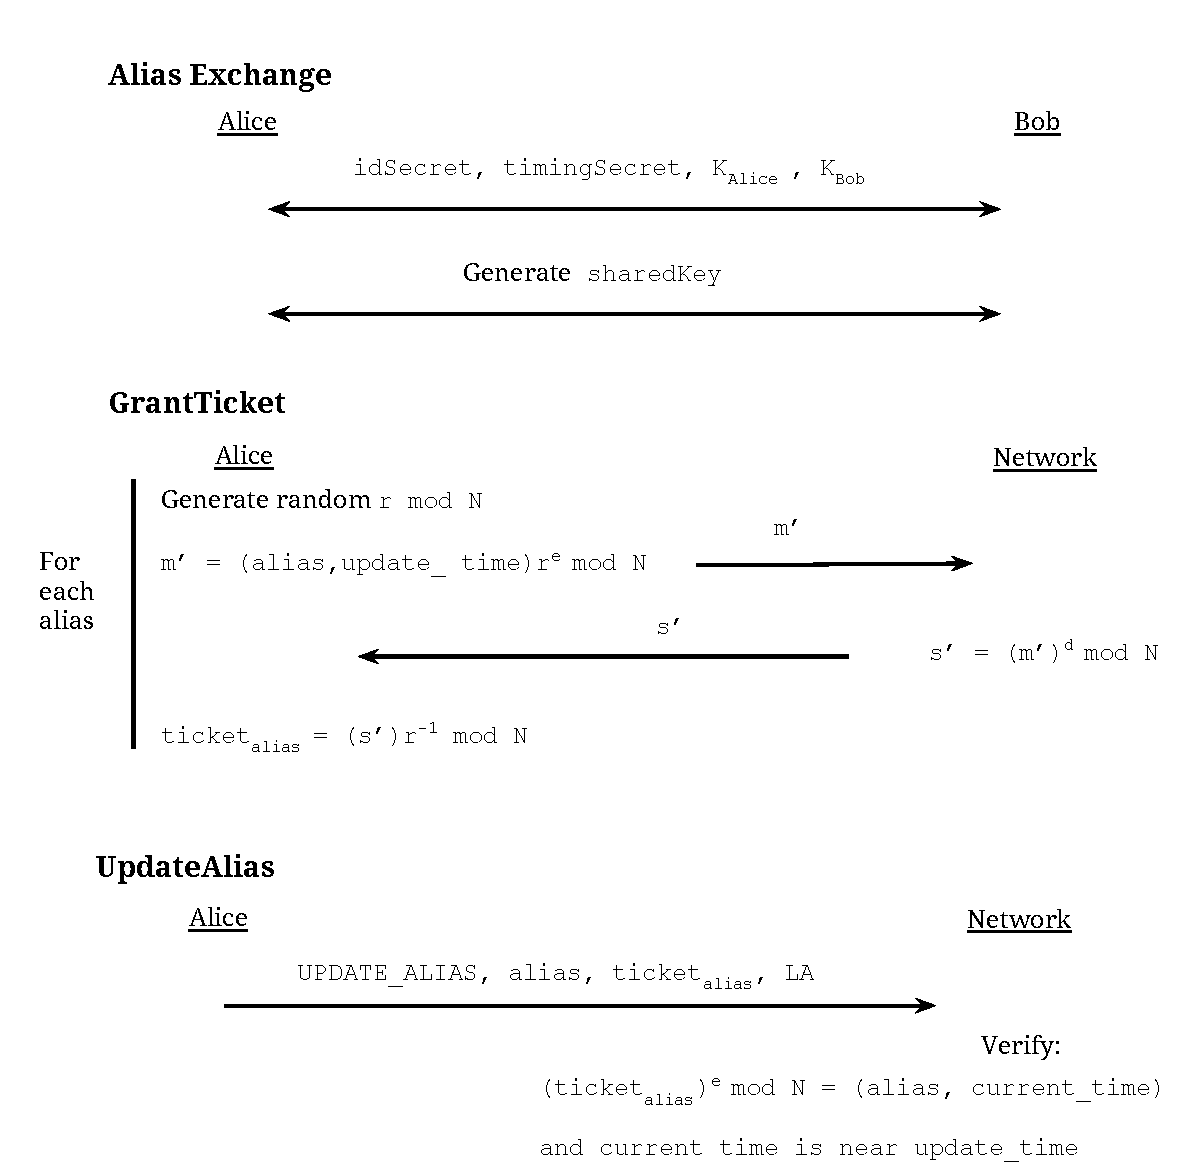
\includegraphics[scale=0.65]{ProtocolsIllustration.pdf}
\end{figure}

\begin{figure}[t]
	\caption{Illustration of \texttt{RequestCall}, and \texttt{AnswerCall} phases.}
	\centering
	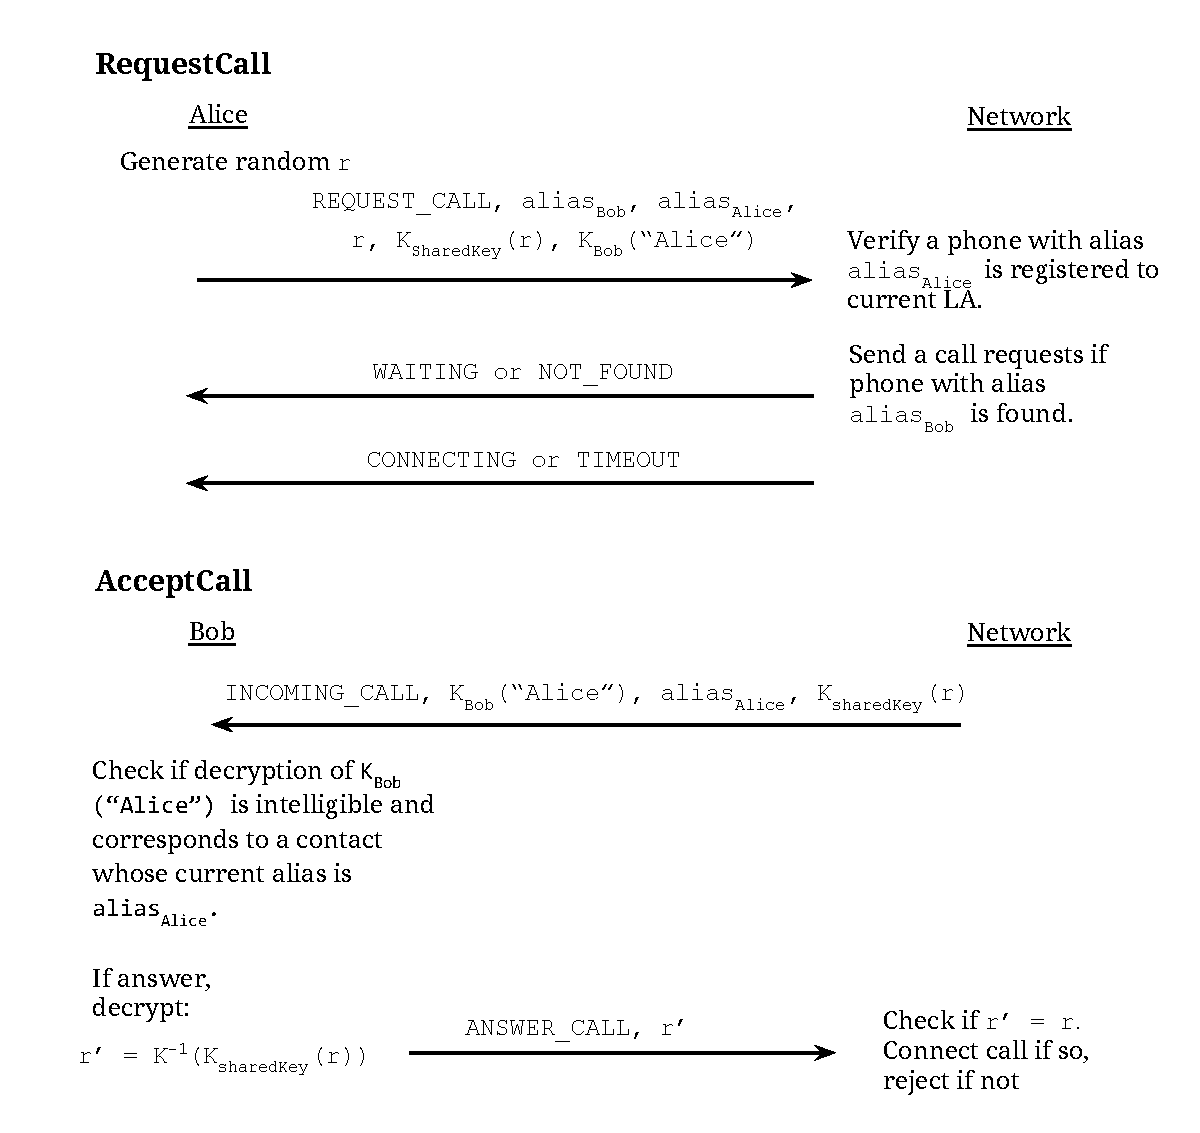
\includegraphics[scale=.65]{ProtocolsIllustration2.pdf}
\end{figure}

\begin{figure}[t]
	\caption{\texttt{GenerateAlias}. In this figure, Bob is computing Alice's current alias in order to make a call.}
	\centering
	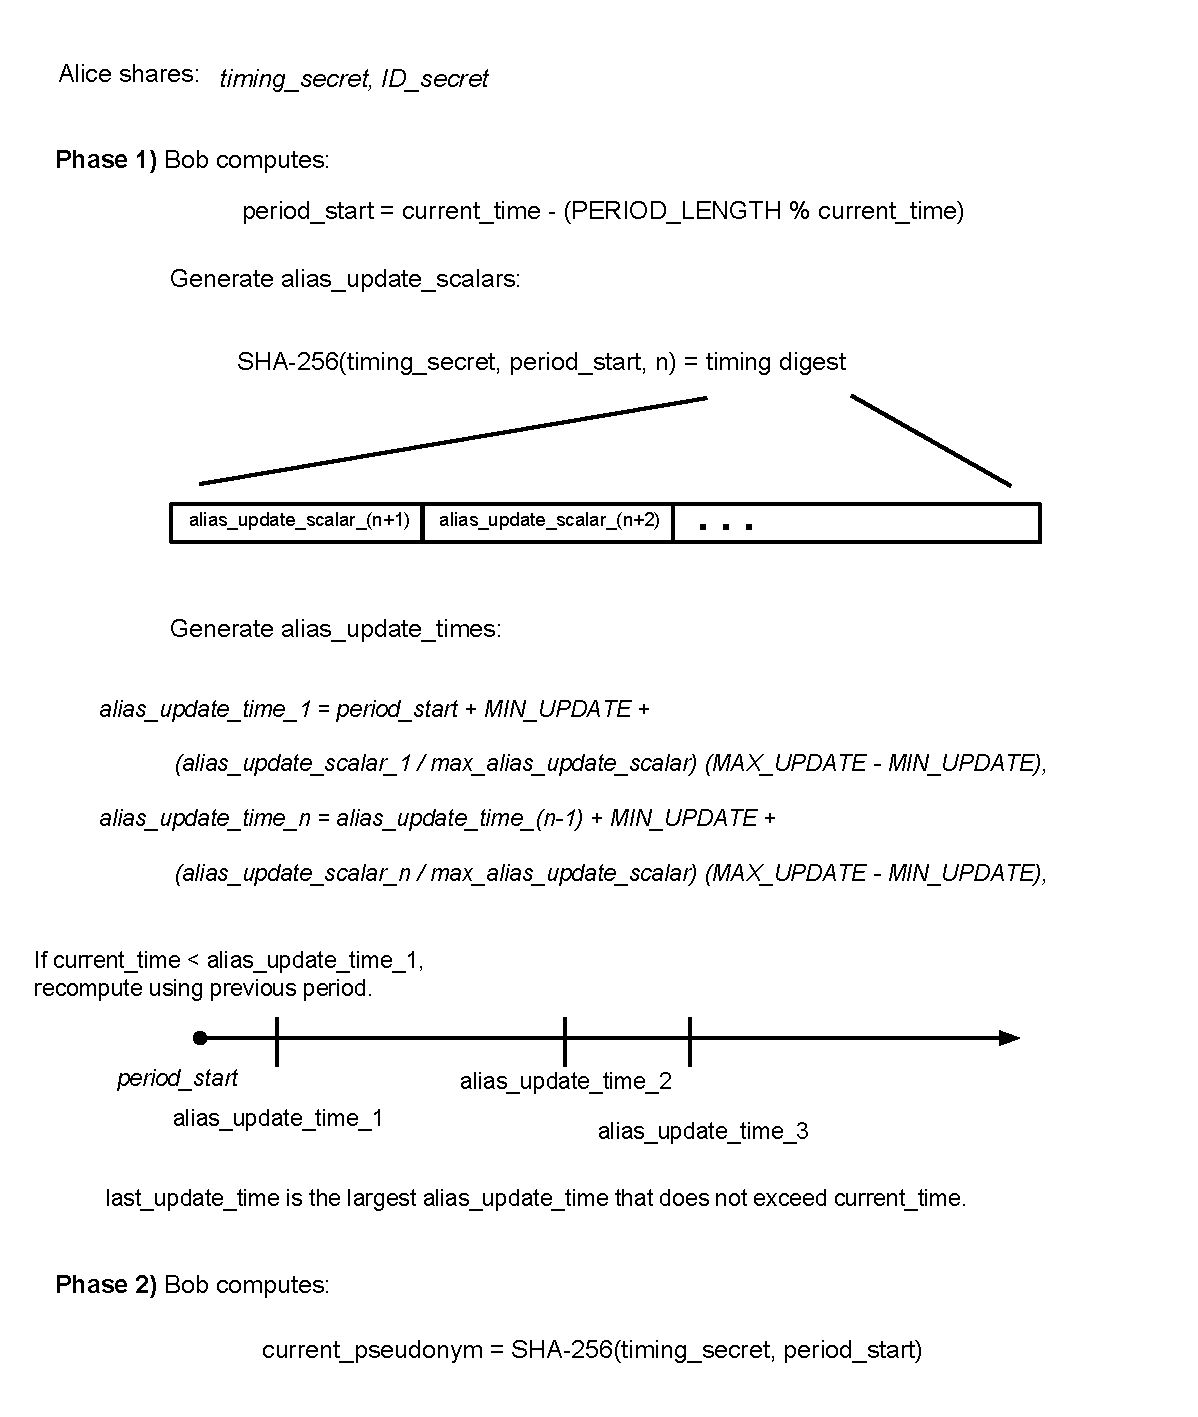
\includegraphics[scale=0.7]{GenerateAlias.pdf}
\end{figure}

\end{document}


